\section{Review Methodology}
\label{sec:methodology}
The review combined broad bibliographic search, automated title-and-abstract screening and provisional classification, and full-text assessment of selected systems. Candidate labels guided discovery; report evidence supported system placements and six detailed comparisons involving twelve systems. Figure~\ref{fig:study-selection-flow} distinguishes records, reports, systems, and placements.

\subsection{Review Scope and Eligibility}
\label{sec:methodology-scope}
The scope is computationally assisted visual analysis of relational and multiscale life-science data. Screening used \emph{bibliographic records} containing titles, available abstracts, and metadata. Full-text assessment used \emph{research reports} to assess the \emph{systems} they describe; several reports can concern one system. At least one system in a report must satisfy all five criteria:

\begin{description}
\item[E1: Life-science application.] Supports analysis, understanding, monitoring, decisions, discovery, or scientific practice in a life-science or closely related domain; training, teleoperation, or presentation alone is insufficient.
\item[E2: Relational or multiscale relevance.] Concerns explicit networks or relationships derived from spatial, temporal, multivariate, image, lineage, similarity, or multiscale data; a network diagram is not required.
\item[E3: Visual-analytics component.] A human uses an interactive or analytically meaningful visual representation to inspect, validate, steer, compare, or interpret data or results; illustration alone is insufficient.
\item[E4: Substantive computational assistance.] A mechanism contributes nontrivially to that workflow, such as clustering, layout, aggregation, annotation, ranking, prediction, or interpreted operations; rendering, pan/zoom, direct parameter entry, or lookup alone does not qualify.
\item[E5: Human analytic relationship.] People inspect, direct, validate, interpret, supervise, correct, or decide from the assisted process; manual control of every operation is not required.

\end{description}

Surveys and general interaction studies provide background and additional discovery routes. Eligibility assessment focuses on reports describing systems and their analytical workflows. Each criterion is assessed using evidence about the same system.

\subsection{Sources and Search Strategy}
\label{sec:methodology-search}
Sources were PubMed, Europe PMC, Semantic Scholar, IEEE Xplore, ACM Digital Library, a local arXiv snapshot, and prior-survey materials. Five overlapping query families covered relational visualization, assisted analysis, interactive systems, nondesktop environments, and conversational analysis. Each combined life-science terms with system, relationship, assistance, or environment terms, including assistance-neutral expressions to retrieve methods without an AI label. Provider syntax and searched fields are documented in the query specifications.

The documented retrieval cutoff was 20 September 2026, with no restriction on the earliest publication date. arXiv identification used a local snapshot containing 3,164,528 records and yielded 958 distinct matches across the query families. Observed snapshot metadata updates extended through 11 September 2026. The snapshot's coverage is considered separately from the cutoff used for the other retrieval routes.

Additional records came from Ehlers-associated working materials, Joos-associated companion material, and a reconstruction of Fonnet and Pri\'e's bibliography, contributing 816, 146, and 207 source occurrences, respectively.~\cite{Ehlers2025,Joos2025VisNetIA,Fonnet2019ImmersiveAnalytics} These records entered the screening workflow alongside database results. The source inventory retains their provenance and distinguishes confirmed survey members, unconfirmed entries, and background references.

\subsection{Deduplication and Source Provenance}
\label{sec:methodology-deduplication}
Deduplication consolidated 187,446 source occurrences into 140,959 bibliographic records using normalized DOI keys, or exact normalized titles when DOIs were absent. Records with and without DOIs remained separate when title agreement was insufficient. Source occurrences and identity decisions were retained, including 50 links between related publication versions. Reports describing the same system were grouped during full-text assessment. The accompanying methods supplement details the identity rules.

\subsection{Title-and-Abstract Screening}
\label{sec:methodology-screening}
Automated screening assessed E1--E5 from titles, available abstracts, and evidence identifiers using the OpenAI Responses API (\texttt{gpt-5.6-luna}, medium reasoning, default service tier, no inference-time browsing or tools). Responses were checked against supplied identifiers and outcomes recomputed locally. \emph{Advance} required support for all five criteria; \emph{Excluded} required evidence against at least one; \emph{Defer} marked insufficient evidence for either decision. Surveys remained background/discovery material, and infrastructure reports were assessed by their described analytical workflow.

Of the 140,959 deduplicated records, 140,810 received valid machine-assisted screening outcomes: 9,505 Advance, 83,258 Defer, and 48,047 Excluded. The remaining 149 records comprise 110 reserved pilot/calibration records, 35 technical failures, and four ambiguous requests that were not resubmitted. Among the excluded records, 10,460 also carried a background-literature flag indicating potential value for context or discovery. This flag is a designation within the excluded set. All 9,505 advanced records proceeded to candidate classification.

\begin{figure*}[t]
\centering
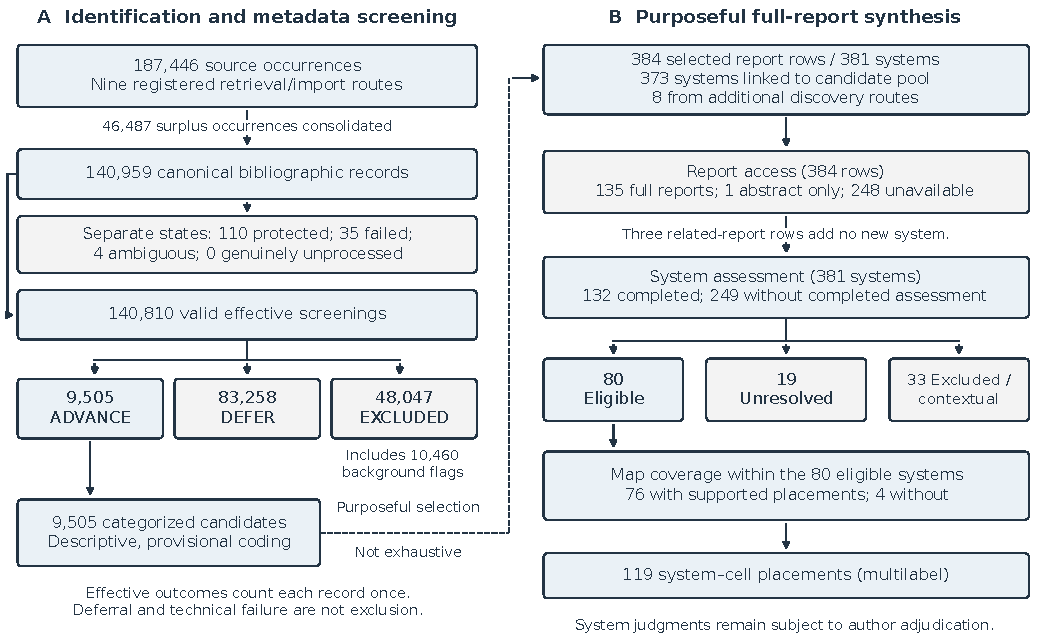
\includegraphics[width=\textwidth]{figures/figure1_selection_flow_119.pdf}
\caption{Identification, screening, and selected-system assessment, reconciled through 26 September 2026. Panel A counts source entries and deduplicated bibliographic records; Panel B distinguishes selected publication entries from the software systems they describe. The dashed handoff denotes selection of systems for detailed assessment. Eight systems entered through coauthor or bounded map-expansion routes without an exact link to the candidate pool. Related reports explain the difference between 135 accessible publication entries and 132 completed system assessments. Multilabel placements are not additional systems. Counts distinguish retrieved records, selected reports, assessed systems, and supported framework placements.}
\label{fig:study-selection-flow}
\end{figure*}

\subsection{Candidate Classification}
\label{sec:methodology-synthesis}
All 9,505 advanced records were provisionally classified from titles and available abstracts using the task, assistance, and modality definitions in Section~\ref{sec:foundations}. Labels could coexist and were recorded as Present, Absent, or Uncertain. These labels guided discovery and selection; supported system-level placements required report evidence for the actual mechanism--environment relationship. The accompanying methods supplement provides the classification contract and candidate co-occurrence table.

\subsection{Full-Text Assessment and Detailed Comparisons}
\label{sec:methodology-assessment}
Systems were selected to compare assistance mechanisms and improve coverage of sparse framework combinations. Six purpose-specific sets contained 20, 18, 50, 200, 24, and 72 report identities. Initial anchors and coauthor reports established comparison cases; bounded queues then prioritized coverage, mechanism and evaluation evidence, and contrasting cases. Software ranked the preliminary shortlist for the 50-entry set, but its final nominations were a separately specified list. The 200-entry queue was selected deterministically by high-precision workflow signal, coverage-rationale class, likely open access, metadata score, and canonical identifier. Software reconciled 25 provisional sparse-cell nominations to 24 entries. The final pass enumerated every exact Present-labelled candidate in three specified cells; scores determined access order, not inclusion. Selector identities and some within-priority rules for the static shortlists are not recorded. The accompanying methods supplement gives the rules, limits, and provenance distinctions for each set.

Assessment used accessible English-language reports to check eligibility, implemented mechanisms, task and modality labels, and evaluation methods and findings. Source passages documented inputs, operations, human intervention, and opportunities to inspect or revise results. Implemented capabilities, measured outcomes, and proposed extensions were recorded separately. The report--system crosswalk traces selection routes, identities, report versions, access, and outcomes.

The selected set comprised 384 publication entries representing 381 systems. Of these, 376 publication entries and 373 systems have exact links to the candidate pool; eight systems were identified through coauthor suggestions or additional searches for framework coverage. Full text was accessible for 135 publication entries, one entry supplied only an abstract, and 248 entries lacked accessible full text. Three accessible entries described related publications about systems already represented, yielding 132 completed system assessments and 249 systems without completed assessments.

Reports describing the same system were grouped using the retained identity crosswalk. Assessments recorded report versions, source passages, and qualifications for each placement. Of the 132 assessed systems, 80 were eligible, 19 remained scientifically unresolved, and 33 were excluded or retained for context. Seventy-six eligible systems supported 119 system--cell placements in Figure~\ref{fig:assistance-modality-map}; four eligible systems lacked a supported placement. A system may occupy several cells because different mechanisms and display environments can coexist. The lead author reviewed and confirmed the placements reported in Figure~\ref{fig:assistance-modality-map}.

A targeted assessment also examined candidate combinations in Immersive--Desktop/Planar, Immersive--Large Display, and Adaptive--Large Display. The 144 candidate memberships resolved to 131 records and 129 system groups, representing 142 distinct system--cell cases. Thirty cases were assessed from full-text reports: 28 lacked support for the proposed placement and two remained unresolved. The other 112 cases were access-limited. This assessment established no additional placements.

Twelve systems were selected for six detailed comparisons to examine how different computational contributions support related analytical work and distribute decisions between scientists and computation. For example, RNA-SeqEZPZ and Facetto illustrate the distinction between configuring an analysis pipeline and teaching a classifier through labeled examples. Compressed Adjacency Matrices and Flud illustrate analyst-controlled organization of a representation versus crowd-assisted optimization of its layout. RetainVis and MediSyn distinguish inspecting model predictions from assessing evidence supporting or contradicting a biomedical interpretation.

Selection considered the availability of reports documenting the mechanisms, human intervention, and evaluation. For each comparison, source passages established the actions performed by computation, the decisions retained or supplied by scientists, and the opportunities to inspect and revise results. These differences informed the evaluation questions developed in Section~\ref{sec:evaluation}. Selection for detailed comparison complemented the broader selection for assistance--modality coverage.

\subsection{Methodological Limitations}
\label{sec:methodology-limitations}
Search coverage depends on provider indexing, query terminology, and the arXiv snapshot's available metadata. The review therefore provides broad candidate discovery and selected-system comparisons rather than an exhaustive enumeration of eligible software. Prior-survey imports add retrieval routes, but coverage of references beyond those imports was not established through systematic recursive citation searching.

Advancement required explicit analytical evidence in titles and abstracts. This favors well-described systems and can defer eligible work with incomplete metadata. Full-text access further affects which systems can be assessed. Selection for framework coverage and detailed comparison supports examination of mechanisms; prevalence estimates would require a different sampling design. The crosswalk traces selected entries, but does not provide a record-by-record reason for leaving every other candidate unselected.

Automated screening and provisional classification were not independently validated across the entire candidate pool. Consequently, the false-exclusion rate, missed eligible systems among deferred records, and pool-wide classification reliability remain unknown. Author confirmation of selected framework placements checks those reported relationships; it cannot establish the accuracy of screening decisions for unreviewed records. Software checks and source verification support consistency and traceability. An independent, stratified review of Advance, Defer, and Excluded records would be needed to estimate screening errors and agreement.

Evaluation studies differ in tasks, datasets, participants, and measures. We compare the benefits and limitations supported within each study's conditions; these heterogeneous findings do not support a pooled effect estimate. The framework's usefulness for researchers has also not been independently evaluated.

\subsection{Supplementary Materials and Use of Generative AI}
\label{sec:methodology-materials}
The software implementing search, deduplication, screening, and evidence management is available at \url{https://github.com/iMammal/h2h-lit-pipeline}. The versioned reproducibility supplement, containing research data, evidence tables, and scripts for regenerating the reported tables and figures, is archived at \url{https://doi.org/10.5281/zenodo.23084434}.

The supplement contains provider-specific query specifications in \texttt{queries/}, retrieval and prior-survey import provenance in \texttt{identification/}, and screening and coding prompts, protocols, and execution settings in \texttt{prompts/}, \texttt{protocols/}, and \texttt{screening/}. The artifact inventory identifies included files and inputs retained outside the public supplement. Raw provider responses, the complete registered corpus, and copyrighted research reports are not redistributed.

\paragraph*{Use of generative AI.}
\label{sec:ai-disclosure}
OpenAI ChatGPT and Codex assisted with literature-processing software, evidence extraction and organization, system comparisons, manuscript drafting and revision, and preparation of LaTeX, tables, and figures. Automated screening and provisional classification used the Responses API as described in Section~\ref{sec:methodology-screening}. Google Gemini contributed preliminary calibration judgments. Checks included software tests, verification of record identities and source passages, deterministic recomputation of screening outcomes, citation checks, and inspection of rendered figures and documents. Reproduced interface images were extracted or cropped from their cited sources. The lead author reviewed all AI-generated content incorporated into the manuscript. The authors retain responsibility for its interpretation, accuracy, attribution, and final content.
